% ----------- tensor_4x4x4.tex -----------
\documentclass[tikz,border=5pt]{standalone}

% TikZ settings ---------------------------------------------------------------
\usepackage{tikz}
\usepackage{amsmath}
\usepackage{amssymb}
\usepackage{color}
\usetikzlibrary{3d,calc}

\makeatletter
\newcommand{\digitTwoPair}[1]{%
  \ifcase#1 % 0 → first branch
    22%
  \or       % 1
    21%
  \or       % 2
    12%
  \or       % 3
    11%
  \else
    \PackageError{digitTwoPair}{Argument must be 0--3}{\@eha}%
  \fi}
\makeatother

\begin{document}
    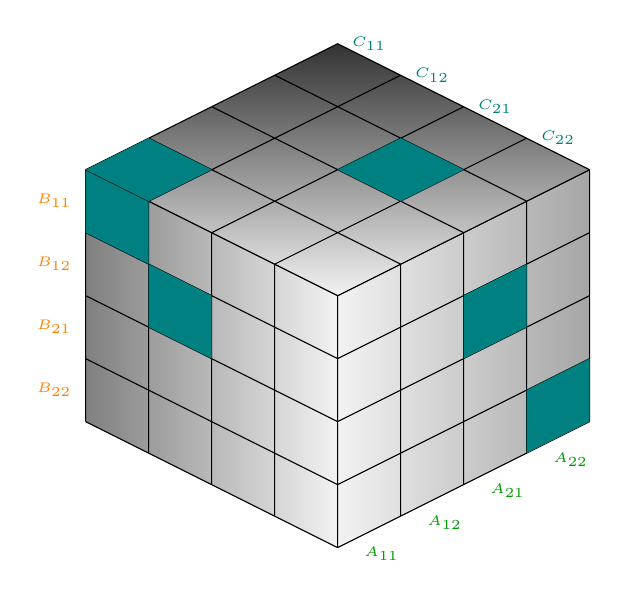
\begin{tikzpicture}[scale=0.8]
        % Front face (4x4 grid)
        \shade[yslant=-0.5,right color=gray!10, left color=black!50]
        (0,0) rectangle +(4,4);
        \draw[yslant=-0.5] (0,0) grid (4,4);
        \fill[teal,yslant=-0.5] (1,2) rectangle +(1,1);
        \fill[teal,yslant=-0.5] (0,3) rectangle +(1,1);

        % Add variables to front face
        \foreach \x in {-1}{
            \foreach \y in {0,1,2,3}{
                \node at (\x+0.5,\y+0.5) {\tiny $\color{orange} B_{\digitTwoPair{\y}}$};
            }
        }

        % Right face (4x4 grid)
        \shade[yslant=0.5,right color=gray!70,left color=gray!10]
        (4,-4) rectangle +(4,4);
        \draw[yslant=0.5] (4,-4) grid (8,0);
        \fill[teal,yslant=0.5] (7,-4) rectangle +(1,1);
        \fill[teal,yslant=0.5] (6,-2) rectangle +(1,1);

        % Add variables to right face
        \foreach \x in {0,1,2,3}{
            \foreach \y in {1}{
              \pgfmathtruncatemacro{\result}{3-\x}
              \node at (4.7+\x,-3.1+\y+\x/2) {\tiny \color{green!60!black} $A_{\digitTwoPair{\result}}$};
            }
        }

        % Top face (4x4 grid)
        \shade[yslant=0.5,xslant=-1,bottom color=gray!10,
            top color=black!80] (8,4) rectangle +(-4,-4);
        \draw[yslant=0.5,xslant=-1] (4,0) grid (8,4);
        \fill[teal,yslant=0.5,xslant=-1] (4,3) rectangle +(1,1);
        \fill[teal,yslant=0.5,xslant=-1] (6,1) rectangle +(1,1);


        % Add variables to top face
        \foreach \x in {0,1,2,3}{
            \foreach \y in {3}{
              \pgfmathtruncatemacro{\result}{3-\x}
                \node at (4+\x+0.5,\y+3.0-\x/2) {\tiny \color{teal} $C_{\digitTwoPair{\result}}$};
            }
        }
        
        

    \end{tikzpicture}
\end{document}
% -------------------------------------------------------------------------------